\documentclass{templateNote}
\usepackage{tcolorbox}
\usepackage{tabularx}
\usepackage{hyperref}
\usepackage{amsmath}
\usepackage{amssymb}
\usepackage{pdflscape}
\usepackage{tikz}
\usepackage{soul}
\usepackage{media9}
\usepackage{adjustbox}
\usepackage{pdfpages}
% \usepackage[spanish,es-noquoting]{babel}

\begin{document}
\linklogoU{https://www.ubiobio.cl/w/}
\linklogoD{https://github.com/NicoxlkboUni}
\imagenlogoU{img/logo-ubb-txt-face.png}
\imagenlogoD{img/logoNGMFormal_sinF.png}
\titulo{Laboratorio 3: Sumador completo}
\asignatura{Laboratorio Arquitectura de Computadores}
\autor{
    Nicolás \textsc{Gómez Morgado}
}

\portada
\margenes

\section*{Ejercicios solicitados}

    
\begin{enumerate}
    \item Escriba algunas oraciones que describan el propósito de este laboratorio. \textbf{10pts}
    \\\\ El propósito de este laboratorio es aprender a diseñar y construir un sumador completo, tanto en software usando Altera Quartus II y ModelSim, 
    como físicamente en una protoboard. Esto nos ayuda a entender mejor la lógica digital y nos prepara para futuros proyectos de diseño de microprocesadores.
    \item Incluya la tabla de verdad completada, incluidos los valores de la columna $C_{out}$. \textbf{10pts}
    \begin{figure}[H]
        \centering
        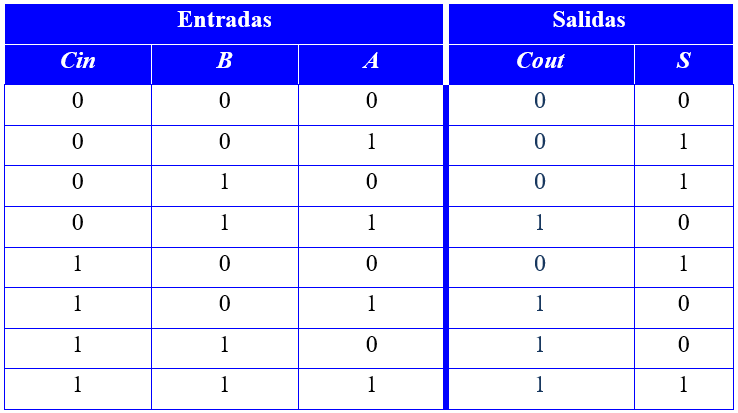
\includegraphics[width=0.5\textwidth]{img/tablaverdad.png}
        \caption{Tabla de verdad del sumador completo}
    \end{figure}
    \item Incluya las siguientes figuras:
    \begin{itemize}
        \item Su esquema completo, incluidas las puertas lógicas para $S$ y $C{out}$. Esto se puede producir utilizando File $\rightarrow$ Export en el Editor de esquemas (es posible que deba seleccionar el formato .bmp). \textbf{20 pts}
        \begin{figure}[H]
            \centering
            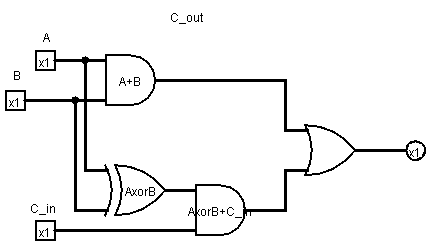
\includegraphics[width=0.5\textwidth]{img/c_out.png}
            \caption{Esquema para $C_{out}$}
            \centering
            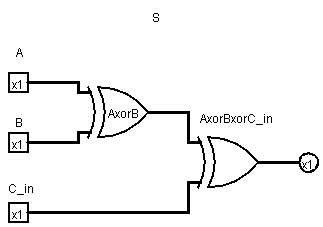
\includegraphics[width=0.5\textwidth]{img/EsquemaS.png}
            \caption{Esquema para $S$}
            \centering
            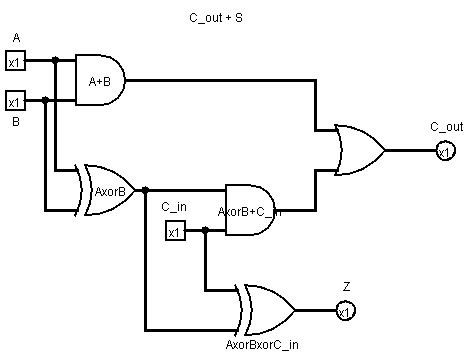
\includegraphics[width=0.5\textwidth]{img/combinacion.png}
            \caption{Combinación de $C_{out}$ y $S$}
        \end{figure}
        \item Su simulación del sumador completo, incluidas todas las entradas y salidas. Esto se puede producir usando File $\rightarrow$ Export $\rightarrow$ Image... característica del simulador ModelSim. \textbf{30pts}
        \begin{figure}[H]
            \centering
            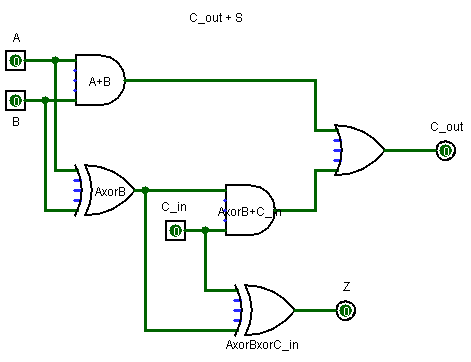
\includegraphics[width=0.5\textwidth]{img/000.png}
            \caption{A = 0, B = 0, $C_{in}$ = 0, $C_{out}$ = 0, $Z$ = 0}
            \centering
            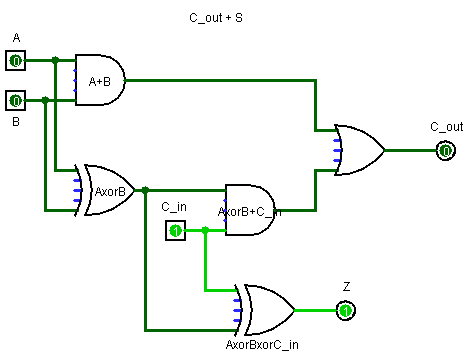
\includegraphics[width=0.5\textwidth]{img/001.png}
            \caption{A = 0, B = 0, $C_{in}$ = 1, $C_{out}$ = 0, $Z$ = 1}
            \centering
            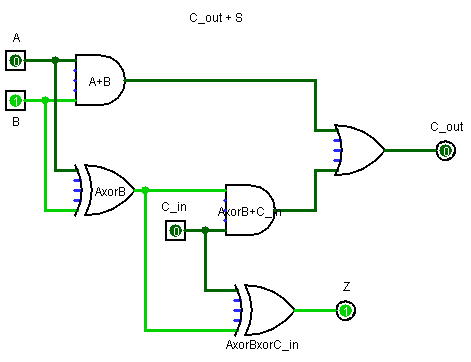
\includegraphics[width=0.5\textwidth]{img/010.png}
            \caption{A = 0, B = 1, $C_{in}$ = 0, $C_{out}$ = 0, $Z$ = 1}
        \end{figure}
        \begin{figure}[H]
            \centering
            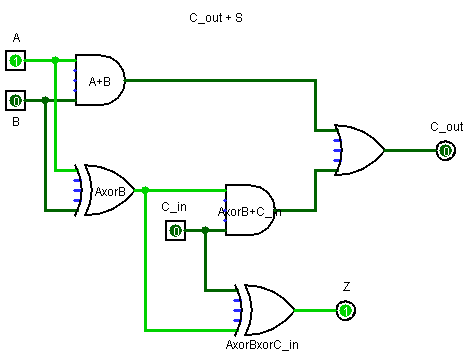
\includegraphics[width=0.5\textwidth]{img/100.png}
            \caption{A = 1, B = 0, $C_{in}$ = 0, $C_{out}$ = 0, $Z$ = 1}
            \centering
            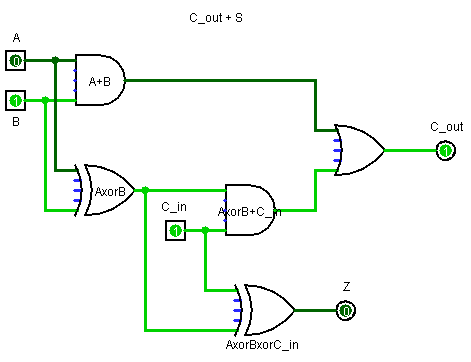
\includegraphics[width=0.5\textwidth]{img/011.png}
            \caption{A = 0, B = 1, $C_{in}$ = 1, $C_{out}$ = 1, $Z$ = 0}
            \centering
            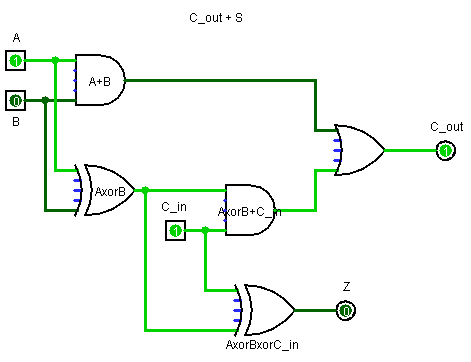
\includegraphics[width=0.5\textwidth]{img/101.png}
            \caption{A = 1, B = 0, $C_{in}$ = 1, $C_{out}$ = 1, $Z$ = 0}
        \end{figure}
        \begin{figure}[H]
            \centering
            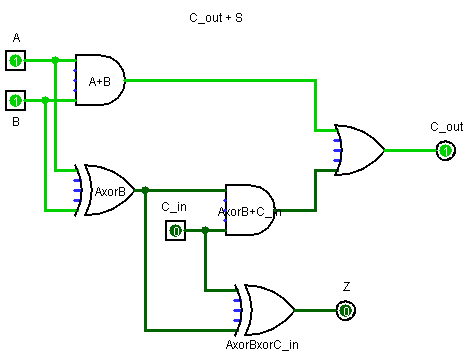
\includegraphics[width=0.5\textwidth]{img/110.png}
            \caption{A = 1, B = 1, $C_{in}$ = 0, $C_{out}$ = 1, $Z$ = 0}
            \centering
            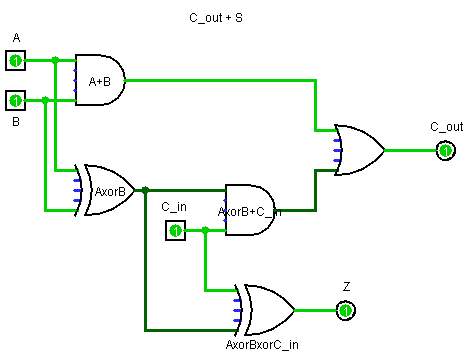
\includegraphics[width=0.5\textwidth]{img/111.png}
            \caption{A = 1, B = 1, $C_{in}$ = 1, $C_{out}$ = 1, $Z$ = 1}
        \end{figure}
        \item Implementación de sumador completo en protoboard (foto de protoboard o captura de Constructor Virtual). \textbf{30 pts}
        \begin{figure}[H]
            \centering
            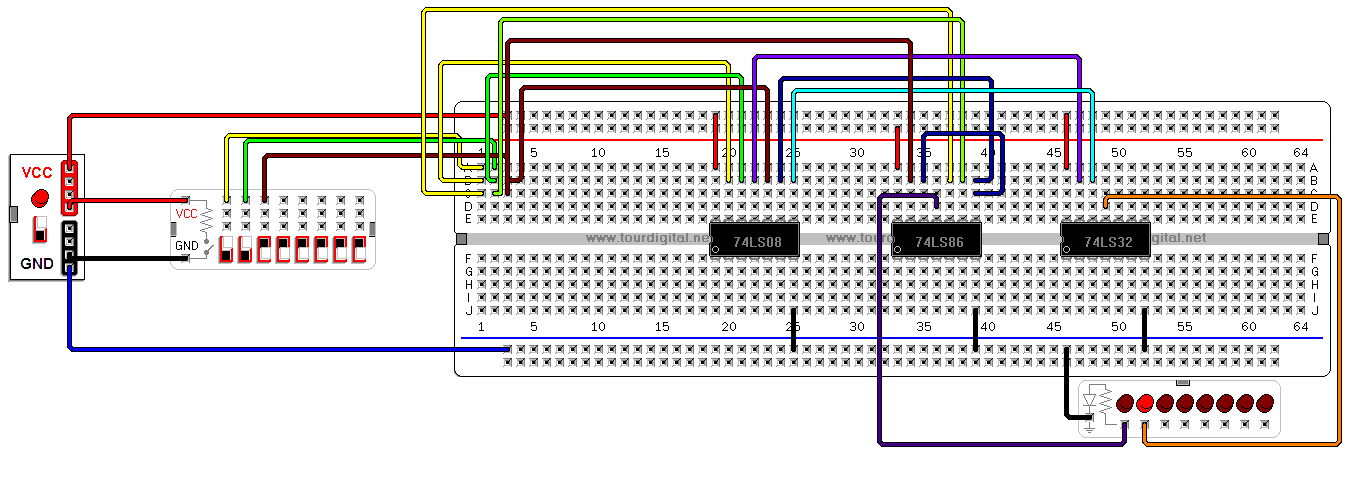
\includegraphics[width=1.0\textwidth]{img/circuitoVirtual.png}
            \caption{Implementación de sumador completo en circuito virtual}
        \end{figure}
    \end{itemize}
    \newpage
    \item ¿Funcionó su sumador completo en el pase de la placa de pruebas para las ocho entradas posibles?
    \\\\ La construcción del sumador en el circuito virtual fue un éxito al momento de obtener los resultados para las ocho entradas posibles en $C_{out}$ y $S$.
\end{enumerate}
% 000
% 001
% 010
% 100
% 011
% 101
% 110
% 111

\end{document}